% !TEX encoding = UTF-8 Unicode
% $Header: /cvsroot/latex-beamer/latex-beamer/solutions/conference-talks/conference-ornate-20min.en.tex,v 1.6 2004/10/07 20:53:08 tantau Exp $

\documentclass[handout]{beamer}
\usepackage{icomma}

% This file is a solution template for:

% - Talk at a conference/colloquium.
% - Talk length is about 20min.
% - Style is ornate.

\mode<presentation>
{
  \usetheme{Warsaw}
  % or ...

  \setbeamercovered{transparent}
  % or whatever (possibly just delete it)
  
  \setbeamertemplate{navigation symbols}{}
  
  \newcommand*\oldmacro{}%
  \let\oldmacro\insertshorttitle%
  \renewcommand*\insertshorttitle{%
    \oldmacro\hfill%
    \insertframenumber\,/\,\inserttotalframenumber}
}

\usepackage[utf8]{inputenc}
% or whatever

\usepackage{times}
\usepackage{multirow}
\usepackage[T1]{fontenc}
\usepackage[french]{babel}
\usepackage{graphicx}
\usepackage{eso-pic}
\usepackage{color}
\usepackage{tikz}
\usepackage{wasysym}

% Or whatever. Note that the encoding and the font should match. If T1
% does not look nice, try deleting the line with the fontenc.

\title[]
{Mangaki.fr, système de recommandation\\de mangas et d'anime}

\author[]
{Jill-Jênn Vie}

\institute[]
{Lycée Thiers}

\date
{16 octobre 2015}

\begin{document}

\definecolor{vert}{rgb}{0.07 0.54 0.07}

{
\setbeamertemplate{headline}[default]
\begin{frame}
	\titlepage
\end{frame}
}

\begin{frame}
	\frametitle{Un système de recommandation}
	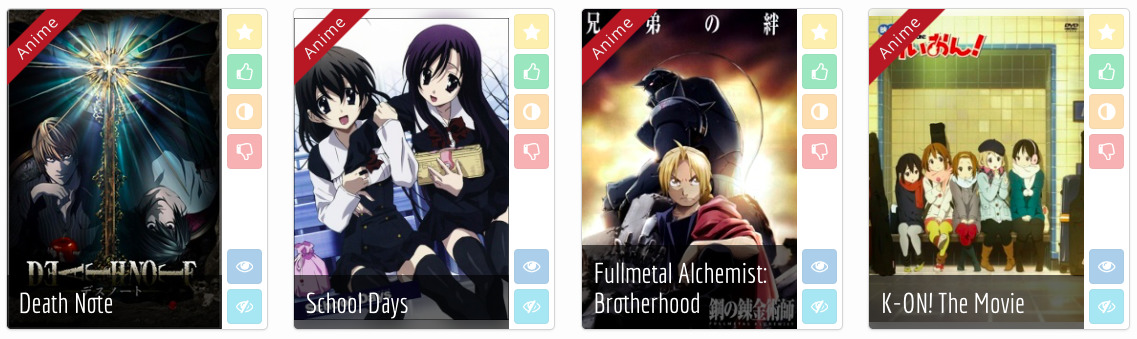
\includegraphics[width=\linewidth]{figures/decks.jpg}
	\begin{block}{Principe}
	\begin{itemize}
	\item Un utilisateur s'inscrit et rentre ses préférences
	\item Le système lui recommande des films susceptibles de lui plaire
	\end{itemize}
	\end{block}
	\pause
	\begin{block}{Objectifs}
	\begin{itemize}
	\item Elles doivent être \alert{pertinentes} (sinon l'utilisateur s'en va)
	\item \alert{Rapides} à calculer (sinon l'utilisateur s'en va)
	\end{itemize}
	\end{block}
\end{frame}

\begin{frame}
	\frametitle{Filtrage collaboratif}
	\begin{block}{Problème}
		\begin{itemize}[<+->]
		\item On dispose d'utilisateurs $u = 1, \ldots, n$\\et d'items à noter $i = 1, \ldots, m$
		\item Chaque utilisateur $u$ attribue une note à une partie des items (\alert{$r_{ui}$} : note de l'utilisateur $u$ sur l'item $i$)
		\end{itemize}
		\pause
		$\Rightarrow$ Quels nouveaux items recommander à chaque utilisateur ?
	\end{block}
	\pause
	\begin{exampleblock}{Exemple (notes sur 5)}
		\begin{tabular}{cccccc}
		& \emph{Death Note} & \emph{L'Attaque des titans} & \emph{Naruto} & \emph{Bleach}\\
		Sacha & ***** & **** & ? & ?\\
		Ondine & ** & ? & * & ?\\
		Pierre & * & ? & **** & ?
		\end{tabular}\\
	\end{exampleblock}
	\pause
	Objets : $n$ vecteurs à $m$ dimensions, éléments de $\{-1, 0, 1\}^m$
\end{frame}

\begin{frame}
	\frametitle{$k$ plus proches voisins}
	\begin{exampleblock}{Intuition}
		\begin{itemize}
		\item On introduit un score de similarité entre utilisateurs
		\item On détermine les $k$ utilisateurs les plus proches d'un utilisateur $u$
		\item On lui recommande ce qu'ils ont aimé qu'il n'a pas vu
		\end{itemize}
	\end{exampleblock}
\end{frame}

\def\R{\mathcal{R}}
\def\N{N}

\begin{frame}
	\frametitle{Produit scalaire}
	Soit $n$ un entier, $u$ et $v$ deux vecteurs de $\mathbb{R}^n$ :
	\begin{itemize}
	\item $u = (u_1, \ldots, u_n)$
	\item $v = (v_1, \ldots, v_n)$
	\end{itemize}\bigskip
	
	Le produit scalaire de $u$ et $v$ est donné par :
	\begin{align*}
	u \cdot v & = u_1 v_1 + \ldots + u_n v_n\\
	& = ||u|| \cdot ||v|| \cdot cos(u, v).
	\end{align*}
\end{frame}

\begin{frame}
	\frametitle{Similarité}
	$\R_u$ : le vecteur de notes $(r_{u1}, r_{u2}, \ldots, r_{um})$ \qquad $u = 1, \ldots, n$\\
	Le \alert{score de similarité} entre 2 utilisateurs $u$ et $v$ est donné par :
	\[ score(u, v) = \R_u \cdot \R_v. \]
	\begin{exampleblock}{Intuition}
	Les points communs augmentent le score :
	\begin{center}
	\begin{tabular}{cccccc}
	& \emph{Paprika} & \emph{Oldboy} & \emph{Gattaca} & \emph{12 Monkeys}\\
	Alice & 1 & -1 & 0 & 0\\
	Bob & 1 & 1 & -1 & 0\\
	Charles & 1 & -1 & 1 & -1
	\end{tabular}\\
	\vspace{5mm}
	$score(Alice, Bob) = 1 + (-1) = 0$\\
%	$score(Bob, Charles) = 1 + (-1) + (-1) = -1$\\
	$score(Alice, Charles) = 1 + 1 = 2$\\
	Alice est \alert{plus proche} de Charles que de Bob.
	\end{center}
	\end{exampleblock}
\end{frame}

\begin{frame}
	\frametitle{Estimation des notes inconnues}
	$\N(u)$ : les $k$ plus proches voisins de $u$, \qquad $u = 1, \ldots, n$\\
	notés $\{v_1, \ldots, v_k\}$\bigskip
	\pause
	\[ \widehat{r_{ui}} = \frac{r_{v_1 i} + \ldots + r_{v_k i}}k \] % \frac1k \sum_{v \in \N(u)} r_{vi} = 
	\pause
	
	On calcule $\widehat{r_{ui}}$ pour chaque film $i$ non noté $\Rightarrow$ les \alert{10 meilleurs}.\bigskip
	
	\pause
	Version \alert{pondérée} : les plus proches ont plus de poids
	\[ \widehat{r_{ui}} = \frac{\sum_{v \in \N(u)} w_v \times r_{vi}}{\sum_{v \in \N(u)} w_v} \quad \textnormal{où } w_v = score(u, v) \]
\end{frame}

\begin{frame}
	Questions :
	\begin{itemize}
	\item Comment choisir la bonne valeur de $k$ dans \og $k$ plus proches voisins \fg ?
	\end{itemize}
	\pause
	Variantes :
	\begin{itemize}
	\item Faire la similarité non sur les utilisateurs sur mais sur les films.
	\end{itemize}
\end{frame}

\begin{frame}
	\frametitle{Évaluation du modèle par validation croisée}
	À quel point j'ai bien recommandé ?
	\begin{itemize}[<+->]
	\item Je suppose que je connais 80 \% des utilisateurs (\alert{\emph{train}})
	\item Je teste les recommandations sur les 20 \% restants (\alert{\emph{test}})
	\end{itemize}\bigskip
	\uncover<4>{Pénalité : les moindres carrés
	\[ RMSE = \sum_{u, i} {(\widehat{r_{ui}} - r_{ui})}^2. \]}
\end{frame}

\begin{frame}
	\frametitle{Une autre méthode : complétion de matrice}
	Supposons que la matrice $M$ de notes soit de \alert{faible rang} $r$ :
	\[ M = \left(\begin{array}{c}
	\R_1\\
	\R_2\\
	\vdots\\
	\R_n
	\end{array}\right) = \raisebox{-1cm}{\begin{tikzpicture}
	\draw (0,0) rectangle (2.5,2);
	\end{tikzpicture}} =
	\raisebox{-1cm}{\begin{tikzpicture}
	\draw (0,0) rectangle ++(1,2);
	\draw node at (0.5,1) {$C$};
	\draw (1.1,1) rectangle ++(2.5,1);
	\draw node at (2.35,1.5) {$P$};
	\end{tikzpicture}} \]
	Chaque ligne $\R_u$ est une combinaison linéaire des lignes de $P$.
	\centering
	$\visible<2->{M : \alert{n} \times \alert{m}} \qquad \visible<3->{C : \alert{n} \times \alert{r}} \qquad \visible<4->{P : \alert{r} \times \alert{m}.}$
	\visible<5->{$\R_1 = c_{11} P_1 + c_{12} P_2 + \ldots + c_{1r} P_r \qquad C_1 = (c_{11}, c_{12}, \ldots, c_{1r})$}
	\visible<6->{\begin{exampleblock}{Exemple}
	\begin{tabular}{@{}lccc@{}}
	Si $P$ & $P_1$ : \og aventure \fg & $P_2$ : \og romance \fg & $P_3$ : \og plot twist \fg\\
	Si $C_u$ & $0,2$ & $-0,5$ & $0,6$
	\end{tabular}
	ça veut dire :\\
	\centering \small j'aime \alert{un peu} l'aventure, je n'aime \alert{pas} la romance,\\
	j'aime \alert{beaucoup} les plot twists.
	\end{exampleblock}}
\end{frame}

\begin{frame}
	\frametitle{Mon sujet de thèse}
	Sur quels items vaut-il mieux sonder un nouveau venu pour le profiler efficacement ?
	\pause
	\begin{itemize}[<+->]
	\item \alert{populaires}, pour que l'utilisateur puisse les noter
	\item \alert{controversés}, pour que ce soit informatif
	\end{itemize}\bigskip
	\uncover<4>{(Arbres de décision, tests adaptatifs.)}
\end{frame}

\begin{frame}
	\frametitle{Quelques liens}
	Merci de votre attention !\bigskip
	\begin{itemize}
	\item mangaki.fr\bigskip\\
	\item jjv@lri.fr
	\end{itemize}\bigskip
	
	\small (P. S. -- C'est la Code Week, apprenez à coder et tentez le concours \alert{Prologin.org}, c'est gratuit et sans obligation d'achat !)
\end{frame}

\end{document}